\documentclass[a4paper, 12pt, addpoints]{exam}
\usepackage[utf8]{inputenc}
\usepackage[english]{babel}
\usepackage{amsmath}
\usepackage{tcolorbox}
\usepackage{graphicx}
\printanswers
\title{\textbf{CG1111A} Tutorial 1}
\author{Prannaya Gupta}
\date{$18^{\text{th}}$ August 2022}
\begin{document}

\maketitle


\begin{questions}
\question Consider the following battery with open-circuit voltage $V_1$ = 12 V, and internal
resistance $R_1$ = 0.15 Ω. Find the load current $I_L$ and the corresponding power efficiency
$\eta_L$ for the following load:

\begin{figure}[h!]
    \centering
    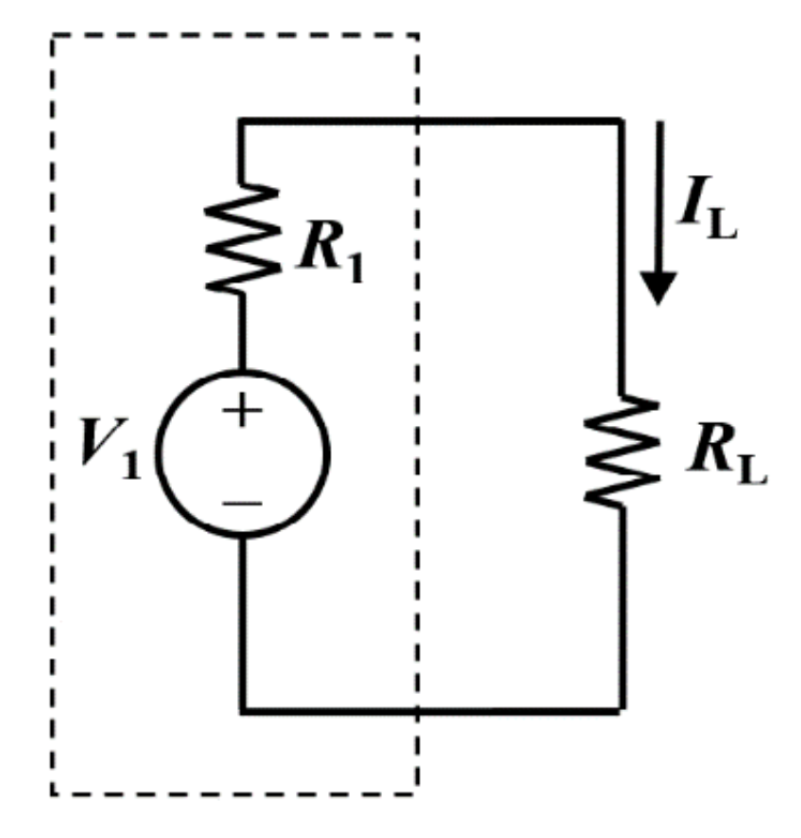
\includegraphics[width=0.3\textwidth]{images/Q1.png}
\end{figure}

\begin{parts}
\part $R_L$ = 10 $\Omega$
\begin{tcolorbox}
\textbf{Solution:}
\begin{align*}
    I_L &= \frac{\varepsilon}{R_T} \\
    &= \frac{V_1}{R_1+R_L} \\
    &= \frac{12}{0.15+10} \\
    &= 1.18227 \\
    &\approx \textbf{1.18 A} \\
    \eta_L &= \frac{P_L}{P_S} \\
    &= \frac{1.18227^2 \times 10}{1.18227\times 12} \times 100\% \\
    &= 98.712\% \\
    &\approx \textbf{98.7\%}
\end{align*}
\end{tcolorbox}

\part $R_L$ = 1 $\Omega$
\begin{tcolorbox}
\textbf{Solution:}
\begin{align*}
    I_L &= \frac{\varepsilon}{R_T} \\
    &= \frac{V_1}{R_1+R_L} \\
    &= \frac{12}{0.15+1} \\
    &= 10.43478 \\
    &\approx \textbf{1.18 A} \\
    \eta_L &= \frac{P_L}{P_S} \\
    &= \frac{10.43478^2 \times 1}{10.43478\times 12} \times 100\% \\
    &= 86.957\% \\
    &\approx \textbf{87.0\%}
\end{align*}
\end{tcolorbox}
\end{parts}    

\question The figure below shows a \textbf{loaded} voltage divider circuit. Calculate the voltage difference $V_\text{AB}$ (given by $V_A - V_B$):

\begin{figure}[h!]
    \centering
    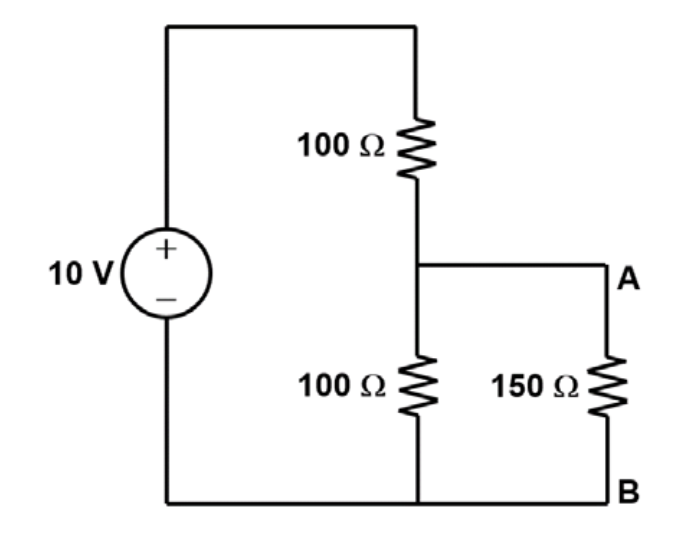
\includegraphics[width=0.3\textwidth]{images/Q2.png}
\end{figure}

\begin{tcolorbox}
    \textbf{Solution:}
    \begin{align*}
        R_\text{AB} &= (\frac{1}{100}+\frac{1}{150})^{-1} \\
        &= 60\text{ }\Omega \\
        R_\text{eff} &= 100 + 60 = 160\text{ }\Omega \\
        I_g &= \frac{\varepsilon}{R_\text{eff}} \\
        &= \frac{10}{160} \\
        &= 0.0625\text{ A} \\
        V_\text{AB} &= I_g \times R_\text{AB} \\
        &= 0.0625 \times 60 \\
        &= \textbf{3.75 V}
    \end{align*}
\end{tcolorbox}

\question Considering the circuit diagram shown in the figure below, which of the following correctly applies \textbf{both} KVL and KCL?
\begin{figure}[h!]
    \centering
    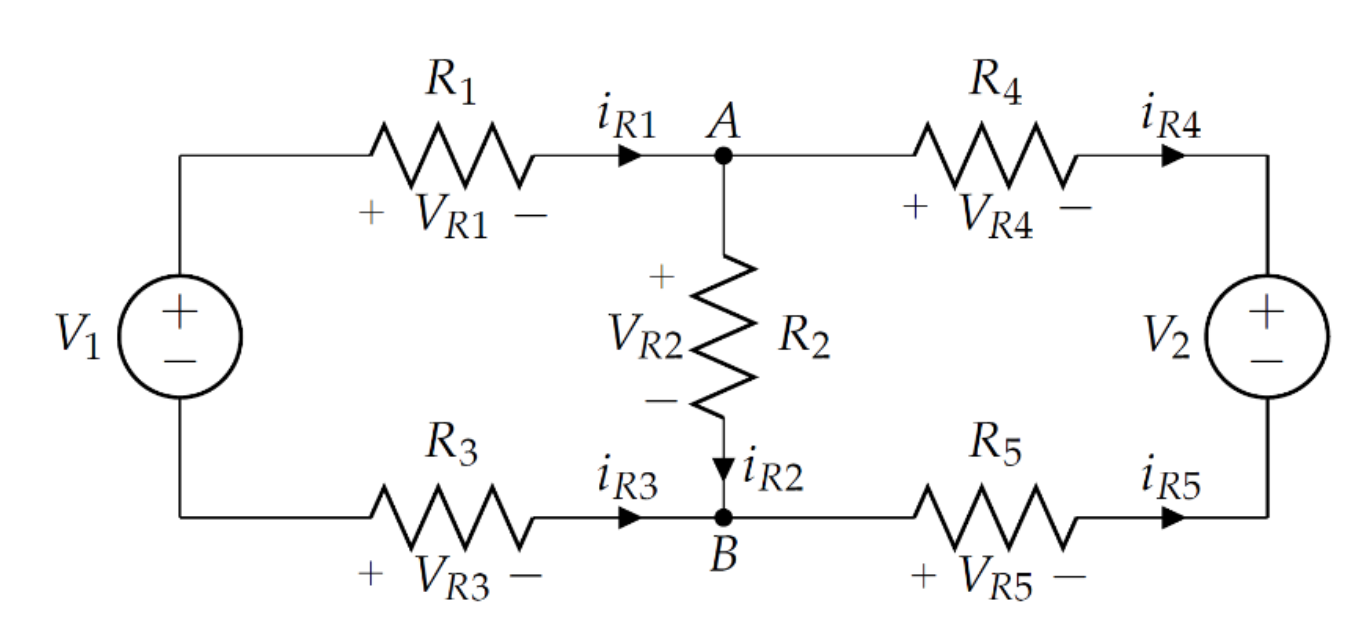
\includegraphics[width=0.7\textwidth]{images/Q3.png}
\end{figure}

\begin{oneparchoices}
    \choice $V_1 - V_\text{R1} - V_\text{R2} - V_\text{R3} = 0$;\quad$i_\text{R1} - i_\text{R2} - i_\text{R4} = 0$ \\
    \choice $V_1 + V_\text{R3} - V_\text{R1} - V_\text{R2} = 0$;\quad$i_\text{R1} + i_\text{R3} = 0$ \\
    \choice $V_2 + V_\text{R4} + V_\text{R2} + V_\text{R5} = 0$;\quad$i_\text{R4} + i_\text{R5} = 0$ \\
    \choice $V_2 + V_\text{R4} - V_\text{R2} - V_\text{R5} = 0$;\quad$i_\text{R3} - i_\text{R2} - i_\text{R5} = 0$
\end{oneparchoices}

\begin{tcolorbox}
    \textbf{Solution: D}
\end{tcolorbox}

\question Determine the source voltage $v$ and the voltage across the 3 $\Omega$ resistor in the following circuit.
\begin{figure}[h!]
    \centering
    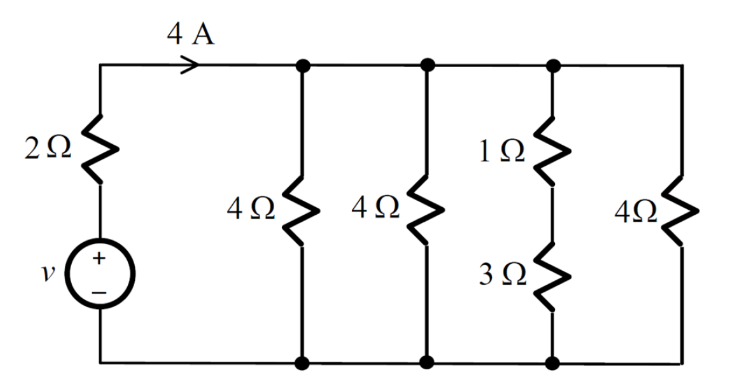
\includegraphics[width=0.7\textwidth]{images/Q4.png}
\end{figure}

\begin{tcolorbox}
    \textbf{Solution:}
    \begin{align*}
        R_{//} &= (3\times \frac{1}{4} + \frac{1}{3+1})^{-1} \\
        &= 1\text{ }\Omega \\
        v &= I_g R_\text{eff} \\
        &= (4)\times (2+1) \\
        &= \textbf{12 V} \\
        V_{//} &= I_g \times R_{//} \\
        &= 4 \times 1 = \text{4 V} \\
        V_{3\text{ }\Omega} &= V_{//} \times \frac{3}{3+1} \\
        &= \textbf{3 V}
    \end{align*}
\end{tcolorbox}

\question THe following circuit shows a common voltage divider for obtaining a certain voltage $v$ across a load resistor $R$.
\begin{figure}[h!]
    \centering
    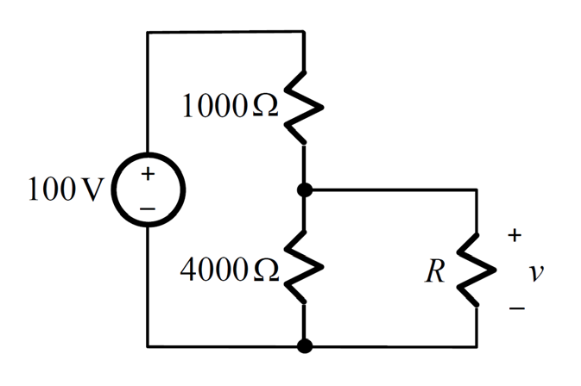
\includegraphics[width=0.5\textwidth]{images/Q5.png}
\end{figure}

A novice may forget to include the loading effects of $R$. To understand these effects, determine $v$ and the current in $R$, $I_R$ when
\begin{parts}
    \part $R = \infty$ (open circuit)

    \begin{tcolorbox}
        \textbf{Solution:}
        \begin{align*}
            R_{//} &= (\frac{1}{4000} + \frac{1}{\infty})^{-1} \\
            &= 4000\text{ }\Omega \\
            V_{//} &= \varepsilon \times \frac{4000}{4000+1000} \\
            v &= 100 \times 0.8 \\
            &= \textbf{80 V}\\
            I_R &= \textbf{0 A}
        \end{align*}
    \end{tcolorbox}

    \part $R = 8000\text{ }\Omega$

    \begin{tcolorbox}
        \textbf{Solution:}
        \begin{align*}
            R_{//} &= (\frac{1}{4000} + \frac{1}{8000})^{-1} \\
            &= \frac{8000}3 \text{ }\Omega \\
            V_{//} &= \varepsilon \times \frac{\frac{8000}3}{\frac{8000}{3}+1000} \\
            v &= 100 \times \frac{8}{11} \\
            &= 72.72727 \\
            &\approx \textbf{72.7 V}\\
            I_R &= \frac{v}{R} \\
            &= \frac{72.72727}{8000} \\
            &= 9.0909\times 10^{-3}\text{ A} \\
            &\approx \textbf{9.09 mA}
        \end{align*}
    \end{tcolorbox}


    \part $R = 200\text{ }\Omega$

    \begin{tcolorbox}
        \textbf{Solution:}
        \begin{align*}
            R_{//} &= (\frac{1}{4000} + \frac{1}{200})^{-1} \\
            &= \frac{4000}{21} \text{ }\Omega \\
            V_{//} &= \varepsilon \times \frac{\frac{4000}{21}}{\frac{4000}{21}+1000} \\
            v &= 100 \times \frac{4}{25} \\
            &= \textbf{16 V} \\
            I_R &= \frac{v}{R} \\
            &= \frac{16}{200} \\
            &= 0.08\text{ A} \\
            &= \textbf{80 mA}
        \end{align*}
    \end{tcolorbox}


    \part $R = 0$ (short circuit)

    \begin{tcolorbox}
        \textbf{Solution:}
        \begin{align*}
            R_{//} &= (\frac{1}{4000} + \frac{1}{0})^{-1} \\
            &= 0 \text{ }\Omega \\
            V_{//} &= \varepsilon \times \frac{0}{0+1000} \\
            &= \textbf{0 V} \\
            I_R &= \frac{\varepsilon-V_{//}}{1000} \\
            &= \frac{100}{1000} \\
            &= 0.1\text{ A} \\
            &= \textbf{100 mA}
        \end{align*}
    \end{tcolorbox}

\end{parts}

\question For the circuit shown in the figure below, what is the value of current $I_1$?
\begin{figure}[h!]
    \centering
    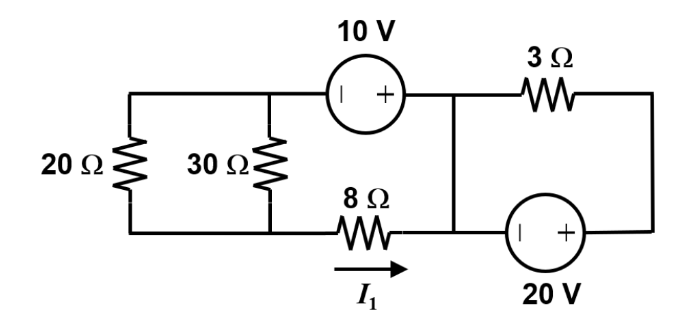
\includegraphics[width=0.7\textwidth]{images/Q6.png}
\end{figure}

\begin{tcolorbox}
    \textbf{Solution:} \\
    Notice that due to the single wire, the 20 V source and the 3 $\Omega$ resistor are in a separate circuit altogether.
    Thus, we only need to simply apply Ohm's Law as follows:
    \begin{align*}
        R_{//} &= (\frac{1}{20} + \frac{1}{30})^{-1} = 12\text{ }\Omega \\
        I &= \frac{\varepsilon}{R_\text{eff}} \\
        -I_1 &= \frac{10}{12+8} \\
        I_1 &= \textbf{-0.5 A}
    \end{align*}
\end{tcolorbox}

\question A current of 3 A flows through a resistor network as shown in the figure below. What is the voltage difference $V_\text{XY}$ (given by $V_X - V_Y$ )?
\begin{figure}[h!]
    \centering
    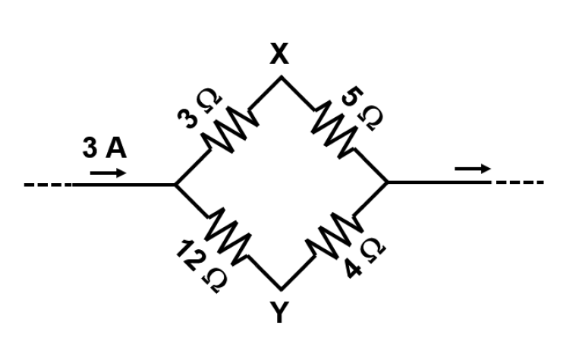
\includegraphics[width=0.5\textwidth]{images/Q7.png}
\end{figure}

\begin{tcolorbox}
    \textbf{Solution:} \\
    Denoting the one above as branch 1, and the one below as branch 2,
    \begin{align*}
        R_{//} &= (\frac{1}{3+5} + \frac{1}{12+4})^{-1} = \frac{16}{3}\text{ }\Omega \\
        I_1 &= I \times \frac{R_{//}}{R_1} = 3 \times \frac{\frac{16}{3}}{3+5} = 2\text{ A}\\
        I_2 &= I \times \frac{R_{//}}{R_2} = 3 \times \frac{\frac{16}{3}}{12+4} = 1\text{A} \\
        V_{3\text{ }\Omega} &= I_1 \times 2 = \text{-6 V} \\
        V_{12\text{ }\Omega} &= I_2 \times 1 = \text{-12 V}\\
        V_\text{XY} &= -6 - (-12) \\
        &= \textbf{6 V}
    \end{align*}
\end{tcolorbox}

\question What is the voltage difference $V_\text{AB}$ (given $V_A - V_B$)?
\begin{figure}[h!]
    \centering
    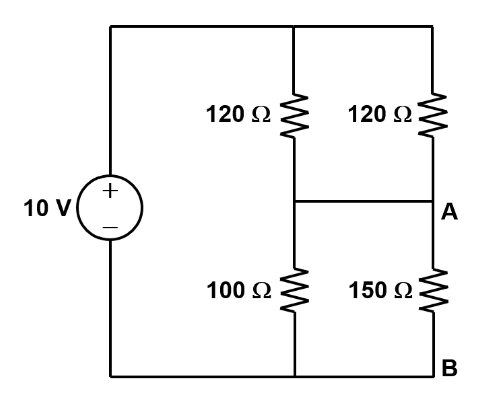
\includegraphics[width=0.5\textwidth]{images/Q8.png}
\end{figure}

\begin{tcolorbox}
    \textbf{Solution:} \\
    This is effectively two parallel sets in series, which can be denoted as $//1$ and $//2$:
    \begin{align*}
        R_{//1} &= (2\times\frac{1}{120})^{-1} = 60\text{ }\Omega \\
        R_{//2} &= (\frac{1}{100}+\frac{1}{150})^{-1} = 60\text{ }\Omega \\
        V_{//2} &= \varepsilon \times \frac{R_{//2}}{R_{//2}+R_{//1}} \\
        V_\text{AB} &= 10 \times \frac{1}{2} \\
        &= \textbf{5 V}
    \end{align*}
\end{tcolorbox}

\question For the circuit shown in the figure below, if the voltage difference $V_\text{BD}$ (given by $V_B - V_D$) is 1 V, what is the value of resistance X?
\begin{figure}[h!]
    \centering
    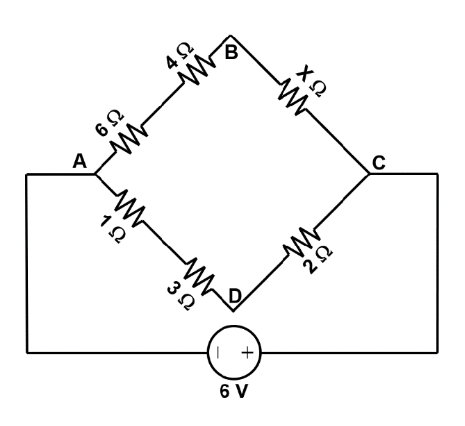
\includegraphics[width=0.5\textwidth]{images/Q9.png}
\end{figure}

\begin{tcolorbox}
    \textbf{Solution:} \\
    Denoting the one above as branch 1, and the one below as branch 2,
    \begin{align*}
        I_1 &= \frac{\varepsilon}{6+4+X} = \frac{6}{10+X} \\
        I_2 &= \frac{\varepsilon}{1+3+2} = 1 \\
        V_{X} &= -I_1 \times X = -\frac{6X}{10+X} \\
        V_{2\text{ }\Omega} &= -I_2 \times 2 = -2\\
        V_\text{BD} &= 2 - \frac{6X}{10+X} \\
        \text{1 V} &= 2 - \frac{6X}{10+X} \\
        \frac{6X}{10+X} &= 1 \\
        6X &= 10 + X \\
        5X &= 10 \\
        X &= \textbf{2 }\bf{\Omega}
    \end{align*}
\end{tcolorbox}

\question The circuit below shows a 10 $\Omega$ load connected to three batteries in parallel. Using node voltage analysis method, determine the voltage across the 10 $\Omega$ load, $V$, and its current $i$.
\begin{figure}[h!]
    \centering
    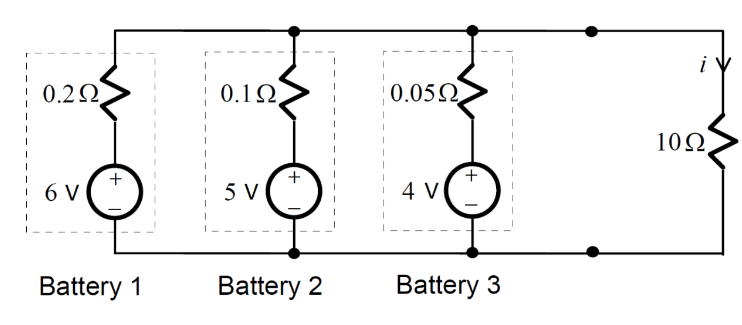
\includegraphics[width=0.7\textwidth]{images/Q10.png}
\end{figure}

\begin{tcolorbox}
    \textbf{Solution:} \\
    Ground the bottom wire. Denote Voltage of top wire as $V$.
    \begin{align*}
        \frac{6-V}{0.2} + \frac{5-V}{0.1} + \frac{4-V}{0.05} &= \frac{V}{10} \\
        300 - 50V + 500 - 100V + 800 - 200V &= V \\
        351 V &= 1600 \\
        V &= 4.55840 \approx \textbf{4.56 V} \\
        i &= \frac{V}{10} \approx \textbf{0.456 A}
    \end{align*}
\end{tcolorbox}

\question For the circuit shown in the figure below, what is the voltage $V_L$? (\textit{Hint: Use Node Voltage Analysis method}) How much power is the 6V source supplying/consuming?
\begin{figure}[h!]
    \centering
    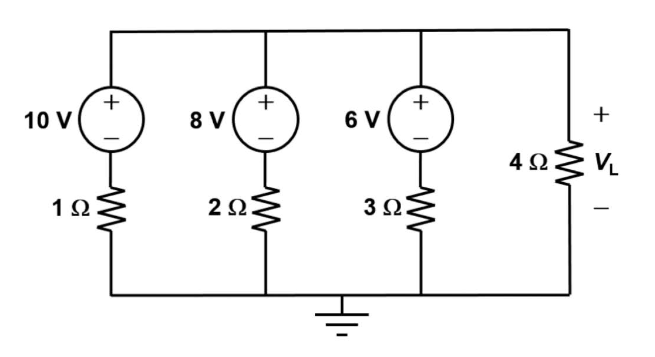
\includegraphics[width=0.7\textwidth]{images/Q11.png}
\end{figure}

\begin{tcolorbox}
    \textbf{Solution:}
    \begin{align*}
        \frac{10-V_L}{1} + \frac{8-V_L}{2} + \frac{6-V_L}{3} &= \frac{V_L}{4} \\
        120 - 12V_L + 48 - 6V_L + 24 - 4V_L &= 3V_L \\
        25 V_L &= 192 \\
        V_L &= \textbf{7.68 V} \\
        I_{6\text{ V}} &= \frac{6-V_L}{3} = -0.56\text{ A}\\
        P &= IV = -0.56 \times 6 \\
        &= \textbf{-3.36 W}
    \end{align*}
    Thus it is consuming \textbf{3.36 W} of power.
\end{tcolorbox}

\question Consider the circuit given below. Suppose $R_5$ is the load resistance, derive and draw the Thevenin equivalent circuit as seen by $R_5$. clearly labeling Node 1 and Node 4 in the equivalent circuit.
(Assume that $R_1 = 1\text{ }\Omega$, $R_2 = 2\text{ }\Omega$, $R_4 = 1\text{ }\Omega$)
\begin{figure}[h!]
    \centering
    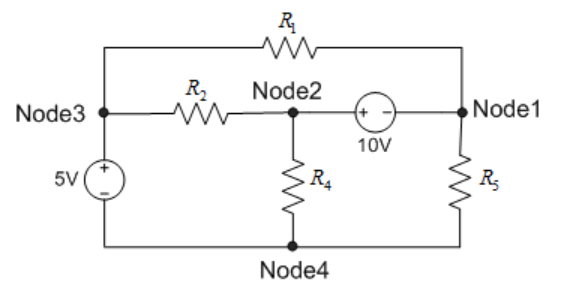
\includegraphics[width=0.7\textwidth]{images/Q12.png}
\end{figure}

\begin{tcolorbox}
    \textbf{Solution:} NO.
\end{tcolorbox}


\end{questions}

\end{document}
